\documentclass[pdflatex,sn-mathphys-num]{sn-jnl}

\theoremstyle{thmstyleone}
\newtheorem{theorem}{Theorem}
\newtheorem{proposition}[theorem]{Proposition}
\newtheorem{corollary}[theorem]{Corollary}
\newtheorem{lemma}[theorem]{Lemma}
\theoremstyle{thmstyletwo}
\newtheorem{remark}{Remark}
\theoremstyle{thmstylethree}
\newtheorem{definition}{Definition}
\newtheorem{assumption}{Assumption}

\usepackage{graphicx}
\usepackage{amsmath,amssymb,amsfonts}
\usepackage{mathtools}
\usepackage{booktabs}
\usepackage{xcolor}
\usepackage{pgfplots}
\pgfplotsset{compat=1.17}

% sn-mathphys-num.bst emits \burl for URLs; route it through hyperref.
\providecommand{\burl}[1]{\url{#1}}

\newcommand{\F}{\mathcal{F}}
\newcommand{\KL}{\mathrm{KL}}
\newcommand{\Bern}{\mathrm{Bern}}
\newcommand{\eps}{\varepsilon}

\raggedbottom

\begin{document}

\title[Semantic Canaries and Partial Unlearning in Unlearning Certificates]{Beyond Planted
Strings: Semantic Canaries, Canary Detectability, and Partial Unlearning in Anytime-Valid
Unlearning Certificates}

% Double-blind toggle: \anontrue for a blinded copy, \anonfalse otherwise.
\newif\ifanon
\anonfalse

\ifanon
\author*[1]{\sur{Anonymous Author}}
\affil*[1]{\orgname{Blinded for review}}
\else
\author*[1]{\fnm{Quang-Vinh} \sur{Dang}}\email{vinh.dq4@buv.edu.vn}
\affil*[1]{\orgname{British University Vietnam}, \orgaddress{\city{Hung Yen},
\country{Vietnam}}}
\fi

\abstract{VOUCH certifies machine unlearning with paired ghost canaries: a fair coin decides which
of two exchangeable records is trained and later unlearned, which makes the sign of their
score difference an exact fair coin under exact unlearning, and betting e-processes turn
these signs into an anytime-valid certificate on the committed cohort. The certificate
was limited to random-string canaries and to a provider trusted not to treat canaries
differently from other data. We extend it in three directions. First, we show that
semantic twins, two incompatible natural-language facts about one fictitious entity drawn
by a label-symmetric generator, keep the exact null for every score that compares the two
facts under the same prompt, including belief scores over paraphrased questions never
seen in training. Second, we prove that the cohort certificate transfers to the generator
population at the cost of a McDiarmid term and to organic records at the cost of twice
the provider's ability to distinguish canaries from organic records, which turns the
honest-provider assumption into a quantitative statement. Every existing canary design is
distinguished with advantage one; twins drawn from the organic record generator with one
slot varied bring perplexity and $n$-gram detectors to chance. Third, on Pythia-410M and
Pythia-1B, unlearning that targets the literal form removes it faster than the fact: the
paraphrase advantage retains $0.21$ more of its pre-unlearning value than the literal one
($p<10^{-6}$ at both sizes), and a union audit over literal and paraphrase scores revokes
up to $38\%$ of the runs that a literal-only audit would certify, while agreeing with it
under no or strong unlearning. BASELINE_SENTENCE We also bound the time at which the cohort
certificate is issued through the growth of the wealth process, exhibiting the
finite-population speed-up.
}

\keywords{machine unlearning, anytime-valid inference, e-values, canaries, membership
inference, large language models}

\maketitle

\section{Introduction}\label{sec:intro}

A user who asks a model provider to delete their data receives, at best, an assurance
that an unlearning routine was run. Whether the routine removed what it was meant to
remove is a statistical question, and VOUCH \citep{dang2026vouch} gave it a statistical
answer. Before fine-tuning, the provider plants \emph{paired ghost canaries}: pairs of
exchangeable records of which a fair coin admits one into training and, later, into
the forget set, while the other is never trained on. Under exact unlearning the deployed
model cannot depend on the coins, so the sign of the score difference between the two
twins is a fair coin, exactly and at any sample size. Betting e-processes built on these
signs give an anytime-valid $(\eps,\alpha)$-forgetting certificate, a revocation alarm,
and a confidence sequence on the residual advantage, with no shadow models and no
retrained reference.

The certificate VOUCH issues has a precise scope: it bounds the realised advantage of a
declared class of scores on the committed cohort of canaries, under a provider that runs
the same pipeline on canaries and on everything else. That scope leaves three questions
open, and each has practical weight.

\emph{First, do canaries stand in for the data users delete?} VOUCH's canaries are
templated records with random secret strings. Users delete biographies, messages and
facts. A certificate on random strings says nothing about natural-language facts unless
something connects the two, and the connection has to survive a provider who might,
deliberately or not, treat the two differently.

\emph{Second, what does a strategic provider need in order to pass the audit without
unlearning?} The honest-but-verifiable threat model of VOUCH assumes the provider does
not special-case the cohort. The assumption is reasonable for an audit run with the
provider's cooperation, but it is an assumption, and the original study measured that
its own canary templates are easy to recognise. How much can a provider gain by
recognising canaries, and what would it take to deny it that gain?

\emph{Third, does an audit of the trained form see knowledge that survives in other
forms?} Gradient-based unlearning has been reported to suppress the exact string it was
given while the fact it encodes stays reachable through a paraphrase
\citep{li2026beliefs}, and a deletion request may name one record of a fact the model
learned from several. A random-string secret has no paraphrase, so
VOUCH's canaries cannot probe this failure. Semantic canaries can, provided the exact
null survives the move to natural language.

\paragraph{Contributions.} This paper extends VOUCH along these three lines, with new
theory and new experiments on Pythia models \citep{biderman2023pythia}.

\begin{itemize}
\item \textbf{Semantic twins keep the exact null.} A twin pair that states two
incompatible facts about one fictitious entity keeps VOUCH's exact conditional null for
every score that compares the two facts under the same prompt, including belief scores
over paraphrased questions that never appear in training, and their versions calibrated
by the base model (Proposition~\ref{prop:semantic}). This realises the natural-language
canary that the original paper named as its next step.

\item \textbf{A ladder from the cohort to organic records.} Under a bounded-influence
assumption, the cohort certificate transfers to the canary generator's population with a
McDiarmid term (Theorem~\ref{thm:population}); and from canaries to organic records with
a term equal to twice the provider's ability to tell the two apart from their contents
(Theorem~\ref{thm:detect}). The second result prices one deviation from the
honest-provider assumption, content-based special-casing: whatever rule a provider uses to
treat canaries differently, the gap it opens is bounded by that rule's distinguishing
advantage (Corollary~\ref{cor:ladder}).

\item \textbf{Detectability and its price, measured.} VOUCH's random-string records and
semantic twins built from their own templates are detected with advantage one by a
character $n$-gram classifier. Twins drawn from the organic record generator itself, with
one slot varied, are not detected by perplexity or $n$-gram detectors beyond the noise of
the detectors. But when such records appear once, as organic records do, Pythia-410M
retains no detectable trace of them, so the audit becomes valid but powerless: the term
the ladder pays for detectability is traded for power (Sections~\ref{sec:exp-detect}
and~\ref{sec:exp-matched}).

\item \textbf{The literal form and the fact under partial unlearning.} When unlearning
targets only the literal statement, the advantage on paraphrased questions is retained
slightly longer than the literal one in all three experiments we ran (two model sizes, two
designs), by $0.07$ to $0.12$ in like-for-like retention; the direction is consistent but
no test reaches significance at eight seeds, so we do not claim to have demonstrated the
squeezing effect at this scale. What does change verdicts is an incomplete forget set:
when the fact was also trained in a form that the forget set does not contain, a union
audit over literal and calibrated paraphrase scores revokes up to $38\%$ of runs that a
literal-only audit certifies, and it costs nothing in validity when the forget set is
complete (Section~\ref{sec:exp-squeeze}).

\item \textbf{Comparison with membership-inference audits.} On the same runs, a
membership-inference test of canaries against an organic holdout raises a false alarm on
every retrained model, because the test detects the difference between canaries and
organic records rather than membership; against matched ghost twins it is valid but
misses partial unlearning that VOUCH's paired, sequential test detects
(Section~\ref{sec:exp-baselines}).

\item \textbf{When the cohort certificate arrives.} Under a uniformly random reveal order
the betting edge of VOUCH's without-replacement process is deterministic
(Lemma~\ref{lem:edge}). A Freedman bound on the wealth process then gives a tail bound on
the certification time that holds before refutation and shows where the
finite-population speed-up comes from (Theorem~\ref{thm:growth}); it is checked
numerically and is conservative by a factor of two to four.
\end{itemize}

All code, results and the scripts that turn results into the tables of this paper are
released with the VOUCH repository.

\paragraph{What is not claimed.} The organic-record result is conditional on the
distinguishing advantage, which data can bound only from below, and on a bounded-influence
assumption that cannot be checked; we report the strongest detectors we could build, not
a proof that none better exists. Squeezing is not demonstrated. All facts in the
experiments are fictitious, the data come from one domain, and the models have at most
one billion parameters and are fine-tuned with LoRA. These limits are discussed in
Section~\ref{sec:discussion}.

\paragraph{Organisation.} Section~\ref{sec:background} recalls VOUCH and fixes notation.
Section~\ref{sec:related} places the work in the literature.
Sections~\ref{sec:semantic}--\ref{sec:time} develop the theory: semantic twins, the
ladder to organic records, and certification time. Section~\ref{sec:experiments} reports
the experiments and Section~\ref{sec:discussion} discusses limitations.

\section{Background: the VOUCH certificate}\label{sec:background}

This section recalls the parts of VOUCH \citep{dang2026vouch} that the extension builds
on and fixes notation; proofs are in the original paper.

\paragraph{Pipeline and threat model.} A provider fine-tunes a model on a corpus,
receives deletion requests, applies an unlearning routine to a forget set, and deploys
the result $M$. An auditor (the verifier) wants evidence that the routine removed the
influence of the forget set. The provider is \emph{honest but verifiable}: it runs the
committed pipeline on the committed data, and in particular processes the canaries
exactly as it processes the rest of the forget set, but it is not trusted to report
whether unlearning succeeded.

\paragraph{Paired ghost canaries.} Before fine-tuning, the verifier generates a cohort of
$m$ pairs with contents $C_i=(c_i^0,c_i^1)$ and draws independent fair coins
$b_i\sim\Bern(\frac12)$. The in-twin $c_i^{b_i}$ is inserted into the training corpus
and later into the forget set; the ghost twin $c_i^{1-b_i}$ is never trained on. The
manifest of contents and coins is committed (VOUCH uses a Merkle commitment), and each
coin is opened only when its pair is audited. All remaining randomness of training and
unlearning is collected in $\xi$.

\paragraph{Scores, signs and the certified quantity.} A score $s(M,c)$ measures how much
the model favours a record, for example the mean token log-probability of a secret
after its prompt. A declared class $\F$ of scores is fixed before any query. For each
pair and score the verifier computes the difference
$D_i^{(s)}=s(M,c_i^{\mathrm{in}})-s(M,c_i^{\mathrm{ghost}})$ and the sign
$Z_i^{(s)}=\mathbf 1[D_i^{(s)}>0]$, ties split by a committed coin. The certified
quantity is the realised cohort advantage
\[
\Delta^{(s)} \;=\; \frac{2}{m}\sum_{i=1}^m Z_i^{(s)} \;-\; 1 ,
\]
which is zero in expectation under exact unlearning and positive when the in-twins are
still favoured. Negative values (the in-twin scores conspicuously below its partner)
are leakage too, and VOUCH certifies both directions.

\paragraph{The exact null.} If $M$ is conditionally independent of the coins given the
contents, which holds for exact unlearning and for retraining from scratch, then for
every score and every step $t$ of a reveal order chosen independently of the signs, the
sign of the pair opened at step $t$ is a fair coin given everything opened before
(VOUCH Theorem~1). No independence across pairs is needed: the signs share one model,
but the coin governing each pair is fair given the past.

\paragraph{The certificate.} The verifier reveals the cohort in a uniformly random order
$\pi$, drawn independently of the signs (VOUCH uses a public randomness beacon), and
for each score and direction runs a betting wealth process
$W_t=\prod_{u\le t}\bigl(1+\lambda_u(p_0(u)-Z_{\pi(u)})\bigr)$ against the
\emph{without-replacement boundary}
\begin{equation}\label{eq:worboundary}
p_0(t) \;=\; \frac{m p_0 - S_{t-1}}{m-t+1},\qquad p_0=\tfrac12+\tfrac\eps2,
\end{equation}
where $S_{t-1}$ is the number of ones revealed before step $t$. If the cohort
advantage were at least $\eps$, the conditional mean of the next sign would be at least
$p_0(t)$, so $W_t$ is a nonnegative supermartingale and Ville's inequality bounds the
probability that it ever reaches $1/\alpha$. A two-sided $(\eps,\alpha)$-certificate is
issued when every per-score, per-direction process has crossed $1/\alpha$, and then
$\Pr[\text{a false certificate is ever issued}]\le\alpha$ under arbitrary dependence
between pairs (VOUCH Theorem~2). If $p_0(t)>1$ the null is infeasible and is refuted
outright. A separate revocation process tests the exact null directly and raises an
alarm (status REVOKED) when it accumulates evidence that the model still depends on the
coins. A run that neither certifies nor revokes ends UNDETERMINED.

\paragraph{Transfer to the coin-averaged advantage.} The cohort advantage depends on the
realised coins. If flipping one coin changes at most $\kappa$ signs, McDiarmid's
inequality \citep{mcdiarmid1989bounded} bounds the distance to the advantage averaged
over the coins with the contents held fixed by $\kappa\sqrt{2\log(2/\alpha')/m}$ (VOUCH
Proposition~3). Section~\ref{sec:organic} extends this transfer to the contents and then
to organic records.

\paragraph{Notation for this paper.} We write $\Delta$ for the cohort advantage of a
fixed score when the score is clear, $\F_t$ for the verifier's filtration after $t$
reveals, and $\mathbb{E}$ for expectation. ``Literal'' refers to scores computed on
the trained surface form of a canary, ``paraphrase'' to scores computed on questions
never seen in training.

\section{Related work}\label{sec:related}

\paragraph{Unlearning methods and their evaluation.} Approximate unlearning for language
models is dominated by gradient ascent on the forget set, negative preference
optimisation \citep{zhang2024npo} and its reference-free variant SimNPO
\citep{fan2025simnpo}, and representation misdirection \citep{li2024wmdp}. They are
evaluated on benchmarks such as TOFU \citep{maini2024tofu} and MUSE \citep{shi2024muse}
whose forget-quality and leakage metrics are fixed-sample statistics compared against a
retrained model. A growing literature shows that these metrics overstate forgetting:
forget-quality metrics track surface behaviour rather than retained knowledge
\citep{wang2025towards}, output matching hides degenerate models \citep{yuan2025closer},
benign relearning restores erased content \citep{hu2025jogging}, relearning attacks can be
formalised and partly resisted \citep{fan2025relearning}, quantisation brings forgotten
knowledge back \citep{zhang2025quantization}, lightweight attacks recover unlearned
capabilities \citep{lucki2024adversarial}, and current evaluations can be made to
overstate or understate success \citep{feng2025existing}; see
\citet{liu2025rethinking} and \citet{xue2026survey} for surveys. Closest to our partial-unlearning experiment, \citet{li2026beliefs}
show that gradient-based unlearning shifts probability mass onto paraphrases of the
targeted answer, which they call squeezing, and propose an objective that accounts for
the model's own beliefs. We study the measurement side of the same phenomenon: whether a
certificate on the trained form can be misled, and what an audit needs to see it.

\paragraph{Membership inference as an audit.} Membership-inference attacks are the usual
instrument of unlearning audits. Score-based attacks threshold the loss, its
zlib-normalised version \citep{carlini2021extracting}, or the mean of the least likely
tokens, Min-K\% Prob \citep{shi2024mink}; reference-based attacks calibrate the loss by a
reference model, and LiRA \citep{carlini2022lira} calibrates per example with shadow
models. \citet{hayes2024inexact} show that unlearning evaluations based on
population-level attacks overstate privacy and that per-example calibration with
shadow models is needed. \citet{zhang2024mia} establish that membership-inference
scores cannot prove that a model was trained on given data unless the inclusion of that
data was randomised, the principle behind VOUCH's fair coins. For pre-trained language
models, \citet{duan2024membership} find that membership-inference attacks perform near
chance when members and non-members are drawn from the same distribution, and
\citet{das2024blind} show that classifiers that never query the model match or beat published
attacks on benchmarks whose members and non-members differ in distribution. Our matched- and
unmatched-holdout baselines (Section~\ref{sec:exp-baselines}) show what happens to a
membership-inference audit when that principle is not respected, and
Theorem~\ref{thm:detect} states the same confound in the language of a certificate.

\paragraph{Verification of unlearning.} \citet{thudi2022necessity} argue that
approximate unlearning cannot be audited from weights alone and that auditable
definitions are a prerequisite for any guarantee; \citet{zhang2024verification} show
that a dishonest provider can defeat existing families of verification strategies while
passing them; cryptographic proof-of-unlearning \citep{eisenhofer2025verifiable} attests
that the committed computation ran, which is complementary to whether forgetting holds
statistically. VOUCH \citep{dang2026vouch} made statistical verification anytime-valid
with paired canaries and betting e-processes
\citep{waudbysmith2024,ramdas2023game,shafer2021testing,grunwald2024safe}, building on
the secret-sharer methodology \citep{carlini2019secret}. Privacy auditing with
canaries \citep{steinke2023privacy} shares the planted design but estimates a lower
bound on the privacy parameter of a training algorithm, not the outcome of one
unlearning run. Copyright traps \citep{meeus2024traps} plant sequences in documents so
that their inclusion in a model's training data can be tested later, a planted design
closer in spirit to ours, without a paired control.
\citet{yu2025impossibility} show that retraining-based definitions of unlearning are not
well posed for multi-stage pipelines, one reason VOUCH avoids a retrained reference.
The special-casing provider that VOUCH's threat model excludes is the subject of
Section~\ref{sec:organic}: we do not remove the assumption, but we price it.

\paragraph{What is new here.} Relative to VOUCH, this paper (i) moves the canaries to
natural language and proves the exact null survives, (ii) states and proves the transfer
from canaries to organic records as a function of canary detectability, and measures
detectability for several designs including one built to make it zero, (iii) tests the
certificate against partial unlearning that suppresses the trained form, with two model
sizes and a union audit, (iv) compares with membership-inference audits on the same
runs, and (v) bounds the certification time through wealth growth rather than through
refutation.

\section{Semantic twins}\label{sec:semantic}

VOUCH's secrets are random alphanumeric strings. A high-entropy string has no
semantically equivalent rephrasing, so a score that reads the secret under paraphrased
carrier sentences finds the same advantage as the literal score, and the squeezing
effect of \citet{li2026beliefs} cannot be observed; the original paper reports exactly
this and names natural-language secrets, exchangeable as propositions rather than as
strings, as the next step \citep{dang2026vouch}. This section defines such
canaries and shows that the exact null survives.

\subsection{The generator}

A semantic twin pair names a fresh fictitious entity $e$ and an attribute $a$ (for
example birthplace or profession) and states two incompatible values of it: $c^0$ says
that $e$ has value $v$, $c^1$ that $e$ has value $v'\neq v$. The pair is drawn by a
generator controlled by the verifier.

\begin{assumption}[Generator]\label{ass:gen}
The pair contents $C_1,\dots,C_m$ are independent draws from a generator distribution
$P$ on ordered pairs that is \emph{label-symmetric}: $(c^0,c^1)\sim P$ implies
$(c^1,c^0)\sim P$. The coins $b_i$ are independent $\Bern(\frac12)$ draws,
independent of the contents and of $\xi$, and $\xi$ is independent of the contents.
\end{assumption}

Both properties are under the verifier's control, because they describe its own
sampler rather than the data or the model. Our generator draws the two values as an
unordered pair from the attribute's value set and swaps them with probability one half,
which makes it label-symmetric by construction; the coins come from a separate random
stream. The in-twin is trained in one or more \emph{training forms}, for example the
literal statement ``$e$ was born in $v$'' and one question--answer form.

\subsection{Scores}

Each score compares the two values under the same prompt, so that both twins of a pair
are scored by the same function of the model:
\begin{itemize}
\item \emph{literal}: the mean token log-probability of the value after the literal
prefix (``$e$ was born in''), $s_{\mathrm{lit}}(M,c^k)=\overline{\log P_M}(v_k\mid
\text{prefix})$;
\item \emph{belief}: the same quantity averaged over a committed set $Q$ of paraphrased
questions (``Where was $e$ born?'', ``What is the hometown of $e$?''), none of which
appears in training;
\item \emph{belief\_max}: the maximum over $Q$ instead of the mean, the semantic
analogue of VOUCH's $s_{\mathrm{para}}$;
\item the \emph{calibrated} version of each, which subtracts the same score computed
under the frozen base model $M_0$: $s^{\mathrm{cal}}(M,c)=s(M,c)-s(M_0,c)$.
\end{itemize}
Calibration removes the base model's prior preference between the two values (a base
model may find ``born in Paris'' more likely than ``born in Porto'' for any name). It
keeps the score in the declared class because $M_0$ is fixed before the coins are drawn.
In the experiments we refer to the literal score as \emph{literal} and to the calibrated
belief scores as \emph{paraphrase}.

\subsection{The exact null}

\begin{proposition}[Exact null for semantic twins]\label{prop:semantic}
Under Assumption~\ref{ass:gen}, if the deployed model is conditionally independent of
the coins given the contents, then for every score $s$ of the form above and every step
$t$ of a reveal order chosen independently of the signs,
$Z_{\pi(t)}^{(s)}\mid\F_{t-1}\sim\Bern(\frac12)$ exactly.
\end{proposition}

\begin{proof}
The proof of VOUCH Theorem~1 uses only that, given the unordered pair opened at step
$t$, the two numbers $s(M,c^0)$ and $s(M,c^1)$ are determined, and that the coin
deciding which of them belongs to the in-twin is fair given everything opened before
and independent of the model given the contents. Neither the semantics of the records
nor the form of $s$ enters, provided $s(M,\cdot)$ is a function of the model and the
record alone. Each score above is such a function: both twins share the prefix or the
question set and differ only in the value evaluated, and the calibrated score subtracts
a function of $M_0$ and the record, where $M_0$ does not depend on the coins.
\end{proof}

Two remarks delimit what the proposition gives. First, \emph{semantics costs power, not
validity}. A base-model prior between the two values enters both arms symmetrically and
leaves the null exact, but it adds variance to the score differences; calibration
removes most of it. Second, the null does not need label symmetry: the coin, not the order of the pair,
decides which twin is trained. Label symmetry matters for what the certificate says
about records outside the cohort. It makes the two components $c^0$ and $c^1$ of a pair
identically distributed, so every canary record is a draw from a single record
distribution, whichever position it occupies and whichever twin the coin trains, and it is this distribution that Section~\ref{sec:organic} compares with
the records users actually delete.

\section{From the cohort to organic records}\label{sec:organic}

The VOUCH certificate concerns the realised advantage $\Delta$ on one committed cohort.
This section climbs a ladder of three targets: the cohort, the generator population,
and organic records, the data users actually delete. Each step costs one term in the
tolerance, and each term has its own cause.

\subsection{From the cohort to the generator population}

VOUCH Proposition~3 averages over the coins with the contents fixed. The verifier also
controls the contents, through Assumption~\ref{ass:gen}, so the same argument reaches
them.

\begin{assumption}[Bounded influence]\label{ass:influence}
For fixed $\xi$, changing a single coin $b_i$ changes at most $\kappa$ of the $m$
signs, and replacing the contents $C_i$ of a single pair changes at most $\ell$ of
them.
\end{assumption}

Under exact unlearning $\kappa=\ell=1$: the model carries no trace of the forget set,
so a pair's coin or contents can affect only that pair's own sign. Under partial
unlearning $\kappa$ and $\ell$ measure how far one canary's training reaches into the
others' scores; they are small for canaries about distinct fictitious entities.

\begin{theorem}[Transfer to the generator population]\label{thm:population}
Let $\Delta_\xi=\mathbb{E}_{b,C}[\Delta\mid\xi]$ be the expected advantage of this
pipeline run over fresh cohorts from $P$. Under Assumptions~\ref{ass:gen}
and~\ref{ass:influence}, for any $\alpha'\in(0,1)$, with probability at least
$1-\alpha'$ over $(b,C)$,
\[
|\Delta-\Delta_\xi| \;\le\; u_m(\alpha') \;:=\;
\sqrt{\frac{2(\kappa^2+\ell^2)\log(2/\alpha')}{m}} .
\]
Consequently a two-sided $(\eps,\alpha)$ cohort certificate implies
$|\Delta_\xi|<\eps+u_m(\alpha')$ with probability at least $1-\alpha-\alpha'$.
\end{theorem}

\begin{proof}
Given $\xi$, $\Delta$ is a function of the $2m$ independent coordinates
$(b_1,\dots,b_m,C_1,\dots,C_m)$. By Assumption~\ref{ass:influence}, changing one coin
changes $\Delta$ by at most $2\kappa/m$ and changing one pair's contents by at most
$2\ell/m$. McDiarmid's inequality \citep{mcdiarmid1989bounded} gives
$\Pr[|\Delta-\Delta_\xi|\ge u]\le 2\exp(-2u^2/\sum_k c_k^2)$ with
$\sum_k c_k^2=4(\kappa^2+\ell^2)/m$, that is
$2\exp\bigl(-u^2m/(2(\kappa^2+\ell^2))\bigr)$; equating it to $\alpha'$ gives $u_m$. The
consequence follows from a union bound with the certificate's error probability.
\end{proof}

$\Delta_\xi$ averages over cohorts but conditions on the training randomness $\xi$: it
is the advantage of \emph{this} deployed pipeline run on the generator population, the
relevant target for an auditor of a deployed model. Averaging over $\xi$ would need
several independent training runs and is not attempted. At $m=512$, $\alpha'=0.05$ and
$\kappa=\ell=1$ the inflation is $u_m=0.17$, against $0.12$ for the coin-only transfer.

\subsection{From canaries to organic records}

Let $P_o$ be a distribution of \emph{organic} record pairs: two records of the kind a
user deletes, with a hypothetical fair coin choosing which one was trained on. For pair
contents $c$, let
\[
h_\xi(c) \;=\; \mathbb{E}\bigl[\,2Z_i-1 \;\big|\; C_i=c,\ \xi\,\bigr]
\]
be the expected sign contribution of a pair with contents $c$ placed in the cohort,
the expectation being over the coins and the other pairs' contents. Then
$\Delta_\xi=\mathbb{E}_{c\sim P}[h_\xi(c)]$, and we define the \emph{organic advantage}
$\Delta^o_\xi=\mathbb{E}_{c\sim P_o}[h_\xi(c)]$: the advantage the same pipeline run
would show on organic pairs planted in the same way. This is the standard notion of
membership leakage under randomised inclusion, evaluated on the data users delete;
because organic records were not in fact included by a coin, it is a counterfactual
quantity of the pipeline, not an observed rate.

\begin{definition}[Distinguishing advantage]\label{def:gamma}
For a class $\mathcal H$ of functions from pair contents to $[0,1]$,
$\gamma_{\mathcal H}(P,P_o)=\sup_{\phi\in\mathcal H}\bigl|\mathbb{E}_P\phi-\mathbb{E}_{P_o}\phi\bigr|$.
When $\mathcal H$ contains all measurable functions, $\gamma_{\mathcal H}$ is the total
variation distance between $P$ and $P_o$.
\end{definition}

\begin{theorem}[Special-casing requires detection]\label{thm:detect}
Let $\phi_\xi=(1+h_\xi)/2$, which takes values in $[0,1]$. Then
\[
|\Delta^o_\xi-\Delta_\xi| \;=\; 2\,\bigl|\mathbb{E}_P\phi_\xi-\mathbb{E}_{P_o}\phi_\xi\bigr|
\;\le\; 2\,\gamma_{\mathcal H}(P,P_o)
\]
for every class $\mathcal H$ that contains $\phi_\xi$. Equivalently, if the pipeline
treats canaries and organic records differently enough to open a gap $g$ between their
advantages, then $\phi_\xi$ is a test that tells canary pairs from organic pairs with
advantage at least $g/2$.
\end{theorem}

\begin{proof}
By linearity, $\Delta_\xi-\Delta^o_\xi=\mathbb{E}_Ph_\xi-\mathbb{E}_{P_o}h_\xi
=2(\mathbb{E}_P\phi_\xi-\mathbb{E}_{P_o}\phi_\xi)$, and the right-hand side is at most
$2\gamma_{\mathcal H}$ in absolute value whenever $\phi_\xi\in\mathcal H$.
\end{proof}

The proof is one line; the content is in the reading. The function $\phi_\xi$ is
computable by anyone who can run the provider's pipeline on a pair and score both
twins, so the relevant class $\mathcal H$ is ``tests the provider can implement''. The
theorem thus turns VOUCH's honest-but-verifiable assumption into a quantitative one: a
provider that special-cases the cohort, unlearning canaries while leaving organic
records untouched, must in effect operate a canary detector, and the gap it can open is
at most twice that detector's advantage. Three consequences follow.

\begin{enumerate}
\item If the manifest is committed but its contents are hidden until after deployment,
the provider can recognise canaries only from their contents, which is what
$\gamma_{\mathcal H}$ measures.
\item An auditor cannot certify $\gamma_{\mathcal H}$ from data. Every detector we train
gives a \emph{lower} bound; none gives an upper bound. We therefore report the strongest
detectors we could build and state the organic claim conditionally on $\gamma$.
\item Making $P$ close to $P_o$ shrinks $\gamma$ against every detector at once. In the
limit where each canary record is drawn from the organic record distribution itself,
$\gamma=0$ at the level of single records.
\end{enumerate}

\begin{corollary}[The ladder]\label{cor:ladder}
Under the assumptions of VOUCH Theorem~2 and of Theorems~\ref{thm:population}
and~\ref{thm:detect}, if a two-sided $(\eps,\alpha)$ cohort certificate is issued, then
with probability at least $1-\alpha-\alpha'$,
\[
|\Delta^o_\xi| \;<\; \eps \;+\; u_m(\alpha') \;+\; 2\gamma_{\mathcal H}(P,P_o).
\]
\end{corollary}

The three terms have separate causes: the tolerance the auditor chose, the size of the
cohort, and how far the canaries are from the data they stand in for. Only the third
depends on the canary design, and Section~\ref{sec:exp-detect} measures it.

\subsection{Organic-matched twins}\label{sec:matched}

The third consequence above suggests a design. Let the organic records be produced by a
generator $G_o$, for example a set of sentence templates with slot distributions, and
draw each canary pair as follows: sample one record $r\sim G_o$, choose one of its slots
(fixed per template), and form the pair by filling that slot with an unordered pair of
values drawn from the slot's distribution and swapped by a fair coin. Each twin is then
a record of $G_o$ with one slot redrawn, so under a slot distribution that is
exchangeable over its values each twin is distributed exactly as an organic record.
We call these \emph{organic-matched twins}. Two details matter. Names are drawn as
in organic data (no distinguishing middle initial), and each canary appears once, since
a record repeated verbatim is itself a signal that organic data rarely gives. The price
is power: a record that looks organic is no easier to memorise than an organic record.

Matching is easy here because we wrote the organic generator. For a deployed model the
organic distribution is the users' own data, and matching it is the hard part of the
problem; Section~\ref{sec:discussion} returns to this.

\section{When the cohort certificate arrives}\label{sec:time}

VOUCH bounds the certification time of the cohort certificate through refutation
(VOUCH Theorem~5): once enough zeros have been revealed, the null becomes infeasible and
is rejected at any level. Refutation is exact but late, since it waits until the
unrevealed remainder cannot carry the null. In practice the wealth process crosses
$1/\alpha$ much earlier, by ordinary growth. This section bounds that time. The key
observation is that under a uniform reveal order the betting edge of the
without-replacement process is deterministic.

\begin{lemma}[Deterministic edge]\label{lem:edge}
Consider the upper certificate arm with $p_0=\frac12+\frac\eps2$. Let the cohort carry
$j$ ones, $\hat p=j/m<p_0$, and $\delta=p_0-\hat p$. Under a uniform reveal order, the
boundary $p_0(t)$ of~\eqref{eq:worboundary} and the conditional mean
$r_t=\mathbb{E}[Z_{\pi(t)}\mid\F_{t-1}]$ satisfy, for every $t$ and every history,
\[
g_t \;:=\; p_0(t)-r_t \;=\; \frac{m\delta}{m-t+1}.
\]
\end{lemma}

\begin{proof}
With $S_{t-1}$ ones revealed, $p_0(t)=(mp_0-S_{t-1})/(m-t+1)$ and, since the unrevealed
remainder is a uniformly ordered set containing $j-S_{t-1}$ ones,
$r_t=(j-S_{t-1})/(m-t+1)$. Subtracting cancels $S_{t-1}$.
\end{proof}

The edge grows as the cohort is exhausted. On an i.i.d.\ stream with the same mean it
would stay equal to $\delta$; the growth is the finite-population advantage of the
cohort target.

\begin{theorem}[Certification time through wealth growth]\label{thm:growth}
Run the upper arm with a uniform mixture of $K$ constant stakes
$\Lambda=\{\lambda_1,\dots,\lambda_K\}\subset(0,\frac12]$, refuting the null outright if
$p_0(t)>1$. Let $H_n$ denote the harmonic numbers,
\[
A_t=\sum_{u\le t}g_u=m\delta\,(H_m-H_{m-t}),\qquad
G_t=\sum_{u\le t}g_u^2=m^2\delta^2\!\!\sum_{k=m-t+1}^{m}\!k^{-2},
\]
and for $\lambda\in\Lambda$
\[
\Psi_t(\lambda)=\lambda A_t-\frac{\lambda^2(t/4+G_t)}{2(1-\lambda)^2},\qquad
V_t(\lambda)=\frac{\lambda^2(t/4+G_t)}{(1-\lambda)^2},\qquad
R_\lambda=\log\frac{1+\lambda}{1-\lambda}.
\]
Then the stopping time $\tau$ of the arm (wealth reaching $1/\alpha$, or refutation)
satisfies, for every $t<m$,
\[
\Pr[\tau>t]\;\le\;\min_{\lambda\in\Lambda}
\exp\!\Bigl(-\frac{x_t(\lambda)^2}{2\bigl(V_t(\lambda)+R_\lambda x_t(\lambda)/3\bigr)}\Bigr),
\qquad x_t(\lambda)=\bigl(\Psi_t(\lambda)-\log(K/\alpha)\bigr)_+ .
\]
\end{theorem}

\begin{proof}
Fix $\lambda\in\Lambda$ and let $X_u=\log\bigl(1+\lambda(p_0(u)-Z_{\pi(u)})\bigr)$,
so that $\log W^\lambda_t=\sum_{u\le t}X_u$. Before refutation $p_0(u)\in[0,1]$, so
$y_u=\lambda(p_0(u)-Z_{\pi(u)})\in[-\lambda,\lambda]$. By Taylor's theorem with
remainder, $\log(1+y)\ge y-y^2/(2(1-\lambda)^2)$ for $y\ge-\lambda$. Hence
$\mathbb{E}[X_u\mid\F_{u-1}]\ge\lambda g_u-\lambda^2\,\mathbb{E}[(p_0(u)-Z_{\pi(u)})^2\mid
\F_{u-1}]/(2(1-\lambda)^2)$, and
$\mathbb{E}[(p_0(u)-Z_{\pi(u)})^2\mid\F_{u-1}]=r_u(1-r_u)+g_u^2\le\frac14+g_u^2$.
Summing over $u\le t$, the compensator of $\log W^\lambda_t$ is at least
$\Psi_t(\lambda)$, a deterministic quantity by Lemma~\ref{lem:edge}. Further,
$|\log(1+y)|\le|y|/(1-\lambda)$ for $|y|\le\lambda$, so the conditional variances of
the $X_u$ sum to at most $V_t(\lambda)$, and the centred increments are bounded below by
$-R_\lambda$. After refutation, replace $X_u$ by its compensator lower bound, so that the
centred sequence remains a martingale difference sequence; this changes nothing on the
event that refutation has not occurred by $t$. Freedman's inequality
\citep{freedman1975tail}, applied to the negated increments, gives
$\Pr[\log W^\lambda_t<\Psi_t(\lambda)-x]\le\exp\bigl(-x^2/(2(V_t(\lambda)+R_\lambda
x/3))\bigr)$. Finally, the mixture wealth is at least $W^\lambda_t/K$, so on the event of
no refutation by $t$ we have $\{\tau>t\}\subseteq\{\log W^\lambda_t<\log(K/\alpha)\}$.
Taking $x=x_t(\lambda)$ and minimising over $\Lambda$ completes the proof.
\end{proof}

\paragraph{Reading the bound.} Since $1/(m-u+1)\ge1/m$, $A_t\ge\delta t$, with equality
only in the limit of an infinite cohort; the factor $\rho_t=m(H_m-H_{m-t})/t\approx
1+t/(2m)$ is the finite-population speed-up. Ignoring $G_t$ and the factor
$(1-\lambda)^{-2}$ and optimising $\lambda$, the drift is about $2\delta^2t\rho_t^2$, so
the time scale is $t^\ast\approx\log(K/\alpha)/(2\delta^2\rho_{t^\ast}^2)$, against
$\log(1/\alpha)/\KL\approx\log(1/\alpha)/(2\delta^2)$ for an i.i.d.\ stream. The original
study found its cohort certificate faster than the super-population one at every
tolerance and attributed this to the cap at cohort exhaustion, where the claim resolves
deterministically. The bound shows that the speed-up starts well before exhaustion,
through the edge that grows as the cohort runs out. The lower arm is the mirror
statement with $\delta'=\hat p-(1-p_0)$, and the two-sided certificate needs both arms.
The theorem covers a constant-stake mixture. VOUCH's engine uses adaptive experts
(online Newton step, Krichevsky--Trofimov); adding the constant-stake grid to the
engine's experts inherits the bound at the cost of $\log$ of the number of experts.

\paragraph{Numerical check.} We compare the bound with the empirical tail of the same
mixture bettor ($K=10$ stakes, $0.05,0.10,\dots,0.50$) over $2{,}000$ uniformly random orders, at $\hat p=\frac12$
and $(m,\eps)\in\{(512,0.2),(1024,0.2),(1024,0.1),(2048,0.1)\}$
(Table~\ref{tab:growth}). The bound is never violated at any of the $32$ checked times
per setting. It is conservative: the first time at which it falls below one half is
$2.2$ to $3.8$ times the empirical median. The same bettor against a fixed boundary on
an i.i.d.\ stream with the same mean is slower in every setting.

\begin{table}[t]
\centering\small
\caption{Certification time of the upper arm, $\hat p=\frac12$, $\alpha=0.05$,
$2{,}000$ uniformly random reveal orders per setting. ``Bound $\le\frac12$'' is the first
checked time at which Theorem~\ref{thm:growth} bounds $\Pr[\tau>t]$ by one half;
``fixed boundary'' is the same bettor on an i.i.d.\ stream with the same mean.}
\label{tab:growth}
\begin{tabular}{rrrrrrr}
\toprule
$m$ & $\eps$ & median $\tau$ & bound $\le\frac12$ & ratio & fixed boundary & violations \\
\midrule
512 & 0.2 & 119 & 346 & 2.9 & 142 & 0/32 \\
1024 & 0.2 & 130 & 490 & 3.8 & 138 & 0/32 \\
1024 & 0.1 & 370 & 810 & 2.2 & 527 & 0/32 \\
2048 & 0.1 & 427 & 1226 & 2.9 & 532 & 0/32 \\
\bottomrule
\end{tabular}

\end{table}

\section{Experiments}\label{sec:experiments}

The experiments ask four questions. How detectable are canaries, and can detectability
be closed by design (Theorem~\ref{thm:detect})? Does an audit with semantic twins
separate memorising from unlearned models on a real language model
(Proposition~\ref{prop:semantic})? Under partial unlearning, does the trained form
disappear before the fact, and does auditing paraphrases change verdicts? How do
membership-inference audits behave on the same runs? Every number below is produced by
a script under \texttt{extension/experiments/}, stored under \texttt{extension/results/},
and turned into the tables of this paper by \texttt{extension/manuscript/make\_tables.py}.
A test suite of eleven tests checks the generators and the exact null without model
weights.

\subsection{Setup}\label{sec:exp-setup}

\paragraph{Data.} The organic records are fictitious biographies drawn from six sentence
templates (birthplace and profession; study city; publication city; years in a city
before a profession; a city guild prize; a workshop near a city) over fictitious first
and last names, cities and professions. These are the keep and forget biographies of the
VOUCH experiments. Each run uses $2{,}000$ keep records, $200$ organic forget records and
a cohort of $m=384$ semantic twin pairs over five attributes (birthplace, profession,
instrument, pet, colour). In-twins are trained in the literal form and one
question--answer form and are repeated $1$, $2$, $4$ or $8$ times by stratum. Belief
scores use four paraphrased questions per attribute, none of which is trained.

\paragraph{Models and training.} The main model is Pythia-410M and the second size is
Pythia-1B \citep{biderman2023pythia}; GPT-2 is used for a pilot and for detector
features. A LoRA adapter \citep{hu2022lora} of rank $16$ on all linear layers is
fine-tuned for $600$ steps (batch $8$, learning rate $2\cdot10^{-4}$, blocks of $96$
tokens). Gradient ascent (GA) and NPO \citep{zhang2024npo} act on a copy of the
fine-tuned adapter with batch $4$ and learning rate $10^{-4}$; NPO uses a retain term on
the keep data and the fine-tuned adapter as its reference. Retraining is a fresh adapter
trained on the keep data only, which satisfies the exact null; no unlearning is the
positive control. All runs were done on single NVIDIA T4 GPUs.

\paragraph{Audit.} Verdicts use the VOUCH engine at $\alpha=0.05$ with a reveal order
drawn from local entropy for the reported runs and from committed seeds for the offline
re-analyses. We report the realised advantage $\hat\Delta$ of the literal score and of
the calibrated belief score (``paraphrase''). Recall that REVOKED rejects the exact null,
some dependence on the coins, at any $\eps$, while ISSUED certifies $|\Delta|<\eps$.

\subsection{Canary detectability}\label{sec:exp-detect}

Theorem~\ref{thm:detect} bounds the gap between canary and organic advantage by twice
the distinguishing advantage $\gamma$. We train two detectors to tell $400$ canary
in-twins from $400$ organic records, both scored out of fold over five folds: a logistic
regression on GPT-2 token-loss features (mean, maximum, median and spread of the token
losses, and length), a trained version of the zero-knowledge perplexity filter of the original study, and a logistic
regression on character $2$--$4$-grams, which requires labelled canaries. A detector's
advantage $\max_\tau|\mathrm{TPR}-\mathrm{FPR}|$ is a lower bound on $\gamma$. For
reference, a detector whose scores are independent of the label exceeds $0.095$ in
$5\%$ and $0.115$ in $1\%$ of $4{,}000$ simulations at this sample size.

\begin{table}[t]
\centering\small
\caption{Detecting canaries among organic records ($400$ canaries, $400$ organic records,
five-fold out-of-fold scores). A detector's advantage is a lower bound on the
distinguishing advantage $\gamma$ of Theorem~\ref{thm:detect}. The null reference for
the advantage is $0.095$ (95th percentile) and $0.115$ (99th).}
\label{tab:detect}
\begin{tabular}{lccccc}
\toprule
 & \multicolumn{2}{c}{Perplexity features} & \multicolumn{2}{c}{Character $n$-grams} & \\
\cmidrule(lr){2-3}\cmidrule(lr){4-5}
Canary design & AUC & advantage & AUC & advantage & $\gamma\ge$ \\
\midrule
VOUCH random-string QA & 0.998 & 0.973 & 1.000 & 1.000 & 1.000 \\
semantic twin, literal & 0.998 & 0.978 & 1.000 & 1.000 & 1.000 \\
semantic twin, question--answer & 0.892 & 0.605 & 1.000 & 1.000 & 1.000 \\
organic-matched twin & 0.521 & 0.052 & 0.442 & 0.102 & 0.102 \\
\bottomrule
\end{tabular}

\end{table}

Table~\ref{tab:detect} compares four designs. VOUCH's random-string records and both forms
of naive semantic twins are detected with advantage one by the $n$-gram classifier, and
the first two also by the zero-knowledge perplexity filter. Random strings, a middle
initial in every canary name and attributes that never occur in organic data give the
cohort away. For these designs Corollary~\ref{cor:ladder} says nothing about organic
records. Organic-matched twins (Section~\ref{sec:matched}) bring both detectors to chance:
the perplexity detector's advantage, $0.052$, is below the 95th percentile of the null
reference, and the $n$-gram detector's, $0.102$, lies between the 95th and the 99th; its
AUC is below one half, so the classifier does not separate the classes in the direction
it was trained for, and the advantage comes from the absolute value in its definition.
These are lower bounds on $\gamma$ against two detector families, not a proof that no
detector exists, which is the conditional nature of Theorem~\ref{thm:detect}. The
original study found that even an entropy-diluted template that defeats the perplexity
filter is still recovered by a trained $n$-gram classifier; matching the organic
generator removes that signature too.

\subsection{Auditing with semantic twins}\label{sec:exp-semantic}

Table~\ref{tab:semantic} audits Pythia-410M when the forget set contains every form the
in-twins were trained in.

\begin{table}[t]
\centering\small
\caption{Semantic-twin audit on Pythia-410M, full forget set ($m=384$, three seeds).
Realised advantages per seed and the two-sided verdict over all scores (I issued, R
revoked, U undetermined).}
\label{tab:semantic}
\begin{tabular}{lllcc}
\toprule
Subject & literal $\hat\Delta$ & paraphrase $\hat\Delta$ & $\eps=0.2$ & $\eps=0.1$ \\
\midrule
no unlearning & $+0.29$, $+0.32$, $+0.46$ & $+0.20$, $+0.27$, $+0.26$ & R R R & R R R \\
GA (100 steps) & $+0.03$, $+0.07$, $-0.05$ & $+0.05$, $+0.05$, $-0.07$ & I I I & I I I \\
NPO (250 steps) & $+0.03$, $-0.09$, $-0.04$ & $+0.07$, $-0.07$, $-0.03$ & I I I & I I I \\
retrain & $-0.03$, $-0.05$, $+0.03$ & $+0.01$, $+0.11$, $+0.08$ & I I I & I U I \\
\bottomrule
\end{tabular}

\end{table}

Paraphrased questions that were never trained carry about two thirds of the literal
advantage, and the audit separates the positive from the negative control in every
seed. A pilot with GPT-2 (128 pairs, 400 training steps) did not: its positive control
reached advantages of $+0.25$ (literal) and $+0.17$ (paraphrase) and was not revoked.
Semantic twins need a model that generalises a stated fact to its paraphrases, which
the smaller model barely does. With the full forget set, GA and NPO remove both
advantages and nothing distinguishes the two scores.

\subsection{Partial unlearning}\label{sec:exp-squeeze}

The case a literal audit cannot see is unlearning that removes the trained surface form
but not the fact. To provoke it we restrict the forget set to the literal statements, so
the question--answer form stays out of it, and sweep the strength of unlearning: GA for
$5$ to $25$ steps and NPO for $10$ to $75$ steps, with eight seeds per model; three of
the Pythia-410M seeds also run GA for $50$ and $100$ steps and NPO for $250$. The
\emph{retention} of a score is its advantage after unlearning divided by the same seed's
advantage before unlearning.

\begin{figure}[t]
\centering
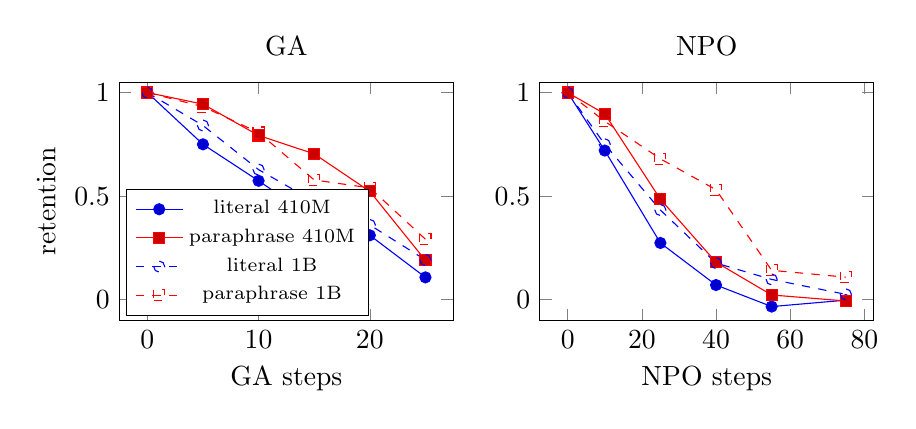
\begin{tikzpicture}
\begin{axis}[name=ga, width=0.48\textwidth, height=0.38\textwidth,
  xlabel={GA steps}, ylabel={retention}, ymin=-0.1, ymax=1.05, title={GA},
  legend style={font=\scriptsize, at={(0.02,0.02)}, anchor=south west}]
\addplot+[mark=*, blue] coordinates {(0,1.000) (5,0.750) (10,0.574) (15,0.391) (20,0.311) (25,0.108)};
\addplot+[mark=square*, red] coordinates {(0,1.000) (5,0.944) (10,0.793) (15,0.704) (20,0.523) (25,0.190)};
\addplot+[mark=o, dashed, blue] coordinates {(0,1.000) (5,0.841) (10,0.628) (15,0.474) (20,0.361) (25,0.192)};
\addplot+[mark=square, dashed, red] coordinates {(0,1.000) (5,0.932) (10,0.807) (15,0.578) (20,0.540) (25,0.292)};
\legend{literal 410M, paraphrase 410M, literal 1B, paraphrase 1B}
\end{axis}
\begin{axis}[at={(ga.east)}, anchor=west, xshift=1.1cm, width=0.48\textwidth,
  height=0.38\textwidth, xlabel={NPO steps}, ymin=-0.1, ymax=1.05, title={NPO}]
\addplot+[mark=*, blue] coordinates {(0,1.000) (10,0.720) (25,0.274) (40,0.071) (55,-0.033) (75,-0.002)};
\addplot+[mark=square*, red] coordinates {(0,1.000) (10,0.897) (25,0.485) (40,0.181) (55,0.023) (75,-0.006)};
\addplot+[mark=o, dashed, blue] coordinates {(0,1.000) (10,0.750) (25,0.433) (40,0.177) (55,0.098) (75,0.026)};
\addplot+[mark=square, dashed, red] coordinates {(0,1.000) (10,0.861) (25,0.680) (40,0.531) (55,0.142) (75,0.109)};
\end{axis}
\end{tikzpicture}
\caption{Retention of the literal and the paraphrase advantage under literal-only
unlearning, mean over eight seeds ($m=384$). Solid: Pythia-410M; dashed: Pythia-1B.}
\label{fig:retention}
\end{figure}

\begin{table}[t]
\centering\small
\caption{Literal-only unlearning on Pythia-410M (top) and Pythia-1B (bottom), eight seeds
each. Advantages are means $\pm$ standard errors; $p$ is the Wilcoxon signed-rank test of
paraphrase minus literal retention (smallest attainable two-sided value $0.008$). The
last two columns count seeds in which the single-score audits disagree at $\eps=0.2$:
A, literal issued and paraphrase revoked; B, the reverse.}
\label{tab:squeeze}
\setlength{\tabcolsep}{4.5pt}
\begin{tabular}{lcccccc}
\toprule
Subject & literal $\hat\Delta$ & paraphrase $\hat\Delta$ & retention lit.\,/\,para. & $p$ & A & B \\
\midrule
none & $+0.363\pm0.026$ & $+0.219\pm0.016$ & 1.00 / 1.00 & -- & 0 & 1 \\
GA 5 & $+0.275\pm0.028$ & $+0.207\pm0.019$ & 0.75 / 0.94 & 0.039 & 0 & 1 \\
GA 10 & $+0.210\pm0.024$ & $+0.175\pm0.020$ & 0.57 / 0.79 & 0.039 & 1 & 1 \\
GA 15 & $+0.143\pm0.016$ & $+0.157\pm0.020$ & 0.39 / 0.70 & 0.008 & 1 & 1 \\
GA 20 & $+0.113\pm0.023$ & $+0.120\pm0.019$ & 0.31 / 0.52 & 0.008 & 2 & 2 \\
GA 25 & $+0.036\pm0.015$ & $+0.038\pm0.016$ & 0.11 / 0.19 & 0.250 & 0 & 1 \\
NPO 10 & $+0.259\pm0.019$ & $+0.195\pm0.020$ & 0.72 / 0.90 & 0.039 & 0 & 0 \\
NPO 25 & $+0.097\pm0.015$ & $+0.109\pm0.022$ & 0.27 / 0.49 & 0.055 & 3 & 1 \\
NPO 40 & $+0.020\pm0.027$ & $+0.046\pm0.026$ & 0.07 / 0.18 & 0.109 & 2 & 0 \\
NPO 55 & $-0.013\pm0.014$ & $+0.007\pm0.028$ & -0.03 / 0.02 & 0.742 & 1 & 0 \\
NPO 75 & $-0.006\pm0.017$ & $+0.005\pm0.021$ & -0.00 / -0.01 & 0.844 & 0 & 0 \\
\bottomrule
\end{tabular}


\vspace{6pt}
\begin{tabular}{lcccccc}
\toprule
Subject & literal $\hat\Delta$ & paraphrase $\hat\Delta$ & retention lit.\,/\,para. & $p$ & A & B \\
\midrule
none & $+0.368\pm0.034$ & $+0.209\pm0.031$ & 1.00 / 1.00 & -- & 0 & 1 \\
GA 5 & $+0.314\pm0.037$ & $+0.199\pm0.033$ & 0.84 / 0.93 & 0.016 & 0 & 4 \\
GA 10 & $+0.241\pm0.038$ & $+0.177\pm0.035$ & 0.63 / 0.81 & 0.055 & 0 & 2 \\
GA 15 & $+0.186\pm0.036$ & $+0.130\pm0.030$ & 0.47 / 0.58 & 0.461 & 0 & 4 \\
GA 20 & $+0.144\pm0.033$ & $+0.116\pm0.020$ & 0.36 / 0.54 & 0.109 & 0 & 2 \\
GA 25 & $+0.072\pm0.026$ & $+0.074\pm0.024$ & 0.19 / 0.29 & 0.461 & 2 & 0 \\
NPO 10 & $+0.283\pm0.040$ & $+0.187\pm0.032$ & 0.75 / 0.86 & 0.008 & 0 & 2 \\
NPO 25 & $+0.166\pm0.032$ & $+0.148\pm0.026$ & 0.43 / 0.68 & 0.008 & 0 & 0 \\
NPO 40 & $+0.073\pm0.023$ & $+0.110\pm0.021$ & 0.18 / 0.53 & 0.008 & 1 & 0 \\
NPO 55 & $+0.039\pm0.020$ & $+0.038\pm0.017$ & 0.10 / 0.14 & 0.641 & 1 & 0 \\
NPO 75 & $+0.008\pm0.012$ & $+0.029\pm0.020$ & 0.03 / 0.11 & 0.383 & 0 & 1 \\
\bottomrule
\end{tabular}

\end{table}

Figure~\ref{fig:retention} and Table~\ref{tab:squeeze} support three findings.

\emph{The literal form is unlearned faster than the fact, at both sizes.} At every
strength where both advantages are still clearly non-zero, paraphrase retention exceeds
literal retention on average. Pooled over GA $10$--$20$ and NPO $25$--$40$ (forty
seed-level cells per model), the mean difference is $0.21\pm0.03$ for Pythia-410M
(positive in $34$ of $40$ cells, Wilcoxon $p=2\cdot10^{-7}$) and $0.21\pm0.04$ for
Pythia-1B (positive in $32$ of $40$, $p=6\cdot10^{-7}$). Before unlearning the paraphrase
advantage is $57$ to $60\%$ of the literal one at both sizes. The effect is largest under
NPO: after $40$ steps on Pythia-1B the literal score retains $18\%$ of its advantage and
the paraphrase score $53\%$, so the literal score understates what survives by a factor
of three. Under GA on Pythia-1B the per-strength differences are smaller, and only the
lightest setting is significant on its own.

\emph{The larger model is harder to unlearn.} At every strength Pythia-1B retains more of
the literal advantage than Pythia-410M (for example $0.43$ against $0.27$ after $25$ NPO
steps), so the strengths at which the literal advantage is small while the paraphrase
advantage is not move towards stronger unlearning: NPO $25$--$40$ for Pythia-410M and
NPO $40$--$55$ for Pythia-1B. A verifier does not know which strength a provider used,
which argues for scoring paraphrases routinely rather than tuning the audit to one
setting.

\emph{Auditing paraphrases changes verdicts where it matters, and only there.}
Single-run verdict counts are noisy here, because two tests near their thresholds
disagree in both directions (columns A and B of Table~\ref{tab:squeeze}). To compare
audit \emph{rules} rather than single runs, we re-run the verifier offline on the stored
score differences of every cell with $40$ reveal orders. Three rules are compared at
$\eps=0.2$, $\alpha=0.05$: the literal score alone; a \emph{union} of two separate
audits, one on the literal score and one on the two calibrated paraphrase scores, each at
level $\alpha/2$, which revokes if either revokes and issues only if both issue, so that
its false-alarm probability under the exact null is at most $\alpha$; and VOUCH's
\emph{mixture} engine over all six scores at level $\alpha$.

\begin{table}[t]
\centering\small
\caption{Fraction of runs (seeds $\times$ $40$ reveal orders) ending REVOKED under three
audit rules, at the strengths where they differ; $\eps=0.2$, $\alpha=0.05$. The last
column is the fraction of runs in which the literal audit issues a certificate and the
union audit revokes.}
\label{tab:union}
\begin{tabular}{llcccc}
\toprule
Model & Subject & literal & union & mixture & lit.\ issued, union revoked \\
\midrule
410M & GA 15 & 0.65 & 0.84 & 0.90 & 0.20 \\
410M & GA 20 & 0.40 & 0.58 & 0.68 & 0.19 \\
410M & NPO 25 & 0.22 & 0.57 & 0.54 & 0.38 \\
410M & NPO 40 & 0.05 & 0.19 & 0.20 & 0.17 \\
1B & GA 15 & 0.63 & 0.66 & 0.65 & 0.04 \\
1B & GA 20 & 0.48 & 0.45 & 0.46 & 0.02 \\
1B & NPO 40 & 0.20 & 0.40 & 0.42 & 0.22 \\
1B & NPO 55 & 0.01 & 0.12 & 0.10 & 0.11 \\
\bottomrule
\end{tabular}

\end{table}

Table~\ref{tab:union} shows the result. With no or light unlearning (none, GA $5$, NPO
$10$) all three rules revoke in at least $97\%$ of runs at both sizes, and with strong
unlearning (GA $\ge50$, NPO $\ge75$) all three revoke in at most $3.3\%$. In between, the
union and the mixture revoke far more often than the literal score alone: after $25$ NPO
steps on Pythia-410M, $38\%$ of runs would issue a literal-only certificate that the
union audit revokes, and after $40$ NPO steps on Pythia-1B, $22\%$. Under GA on Pythia-1B
the rules do not differ, consistent with its small retention gap. The paraphrase scores
are weaker on their own: on the positive control the paraphrase audit alone revokes in
$7$ of $8$ seeds at both sizes. They therefore belong next to the literal score in the
declared class, not in its place, and adding them costs a few forward passes per pair.

\subsection{Comparison with membership-inference audits}\label{sec:exp-baselines}

The usual way to audit unlearning is a membership-inference test: score the forget set and
a holdout set with an attack and ask whether the two are distinguishable, as in the
PrivLeak metric of MUSE \citep{shi2024muse}. We run this test on the literal-only design
(the runs of Table~\ref{tab:clean}), with four membership scores computed on whole records:
the loss, Min-K\% Prob with $k=20\%$ \citep{shi2024mink}, the zlib ratio
\citep{carlini2021extracting}, and the loss minus the base model's loss (``ref''). A test
declares leakage when the $95\%$ bootstrap interval of the AUC excludes $0.5$. Four
pairings of members and non-members are compared: (a) canary in-twins against their ghost
twins, the matched holdout that VOUCH's design provides; (b) canary in-twins against
organic holdout records, the usual holdout of a benchmark; (c) the paraphrased questions
of in-twins against those of ghost twins; and (d) the organic forget biographies against
the organic holdout, the audit on the data users actually delete. To separate the
contribution of pairing from that of sequential testing we add a paired fixed-sample test:
a two-sided sign test at level $0.05$ on the literal score differences of all $384$ pairs,
the same pairs and the same score that VOUCH uses, evaluated once at the end.

\begin{table}[t]
\centering\small
\caption{Fraction of seeds (VOUCH: of seeds $\times$ $40$ reveal orders) in which each audit
reports leakage, literal-only design, Pythia-410M, eight seeds. VOUCH columns are
REVOKED rates of the literal and the union rule; ``sign'' is the fraction of seeds in which
the paired fixed-sample sign test on the literal score rejects; membership-inference
columns are fractions of seeds whose $95\%$ bootstrap AUC interval excludes $0.5$. Retraining is the
exact null, so every positive entry in its row is a false alarm.}
\label{tab:baselines}
\setlength{\tabcolsep}{3.2pt}
\footnotesize\setlength{\tabcolsep}{3pt}\begin{tabular}{l ccc cccc cc cc cc}
\toprule
 & \multicolumn{2}{c}{VOUCH} & sign & \multicolumn{4}{c}{(a) canaries vs.\ ghosts} & \multicolumn{2}{c}{(b) vs.\ organic} & \multicolumn{2}{c}{(c) paraphrase} & \multicolumn{2}{c}{(d) organic} \\
\cmidrule(lr){2-3}\cmidrule(lr){4-4}\cmidrule(lr){5-8}\cmidrule(lr){9-10}\cmidrule(lr){11-12}\cmidrule(lr){13-14}
Subject & lit. & union & lit. & loss & Min-K\% & zlib & ref & loss & ref & loss & ref & loss & ref \\
\midrule
none & 1.00 & 1.00 & 1.00 & 1.00 & 1.00 & 1.00 & 0.75 & 1.00 & 1.00 & 0.00 & 0.00 & 0.38 & 0.12 \\
retrain & 0.02 & 0.01 & 0.00 & 0.00 & 0.00 & 0.00 & 0.00 & 1.00 & 1.00 & 0.00 & 0.00 & 0.12 & 0.00 \\
\midrule
GA 10 & 0.96 & 0.96 & 1.00 & 0.38 & 0.00 & 0.25 & 0.12 & 1.00 & 1.00 & 0.00 & 0.00 & 0.00 & 0.00 \\
GA 15 & 0.68 & 0.67 & 0.88 & 0.00 & 0.00 & 0.00 & 0.00 & 1.00 & 1.00 & 0.00 & 0.00 & 0.25 & 0.00 \\
GA 20 & 0.25 & 0.25 & 0.25 & 0.00 & 0.00 & 0.00 & 0.00 & 1.00 & 1.00 & 0.00 & 0.00 & 0.12 & 0.00 \\
NPO 25 & 0.36 & 0.34 & 0.62 & 0.00 & 0.00 & 0.00 & 0.00 & 1.00 & 1.00 & 0.00 & 0.00 & 0.12 & 0.00 \\
NPO 40 & 0.06 & 0.04 & 0.00 & 0.00 & 0.00 & 0.00 & 0.00 & 1.00 & 1.00 & 0.00 & 0.00 & 0.00 & 0.00 \\
NPO 75 & 0.01 & 0.00 & 0.00 & 0.00 & 0.00 & 0.00 & 0.00 & 1.00 & 1.00 & 0.00 & 0.00 & 0.25 & 0.12 \\
\bottomrule
\end{tabular}

\end{table}

Table~\ref{tab:baselines} shows four things.

\emph{An unmatched holdout makes the test meaningless.} Pairing (b) reports leakage on
every seed of every subject in the table, retraining included (and on seven of eight
seeds after $25$ GA steps), with AUC $0.000$ on retraining: the
canaries and the organic holdout differ in distribution, so the test detects the
difference between two kinds of record, not membership. Calibrating by the base model does
not help. This is the confound of Theorem~\ref{thm:detect} seen from the side of the
attack, and the reason \citet{zhang2024mia} require randomised inclusion; it matches the
observations of \citet{duan2024membership} and \citet{das2024blind} for pre-trained
models.

\emph{A matched holdout restores validity but not power.} Pairing (a) uses the same
records as VOUCH and is valid: no false alarm on retraining, and the positive control is
detected in every seed by the loss, Min-K\% and zlib scores (AUC $0.59$). But under partial
unlearning it falls silent long before VOUCH does: after $10$ GA steps the loss test flags
$38\%$ of seeds where VOUCH revokes $96\%$ of runs, and after $15$ GA steps or $25$ NPO
steps it flags none where VOUCH revokes $68\%$ and $36\%$. The paired fixed-sample sign test on the same pairs is at least as powerful as VOUCH at all
strengths but one (for example $62\%$ of seeds against $36\%$ of runs after $25$ NPO steps;
after $40$ NPO steps it rejects in no seed while VOUCH revokes $6\%$ of runs), so the gap between
VOUCH and the matched-holdout test comes from pairing and from scoring the target value
rather than the whole record, not from sequential testing. An unpaired AUC compares
in-twins with ghost twins across different entities, whose whole-record losses are
dominated by the entities themselves; a paired test compares the two twins of one entity,
which cancels that variation. Sequential testing costs some power against a test run once
at the end, and buys the right to monitor continuously and stop at any time without
inflating the error; the original paper measures what a fixed-sample test loses under
optional stopping.

\emph{The paraphrase and organic audits are weak.} Pairing (c) detects nothing, not even on
the positive control, because a whole-record loss over a question and a one-word answer is
dominated by the question. Pairing (d), the audit on the organic forget set itself, reaches
an AUC of $0.55$ on the positive control and flags it in three of eight seeds, with one
false alarm in eight on retraining; at this training budget a single exposure leaves too
little trace in an organic record for a fixed-sample test to see reliably.


\section{Discussion and limitations}\label{sec:discussion}

\paragraph{What the extension changes in practice.} Three recommendations follow for a
verifier who audits with VOUCH. First, canaries should be drawn from the distribution
of the records they stand in for, because every design that departs from it visibly is
detected with advantage one and leaves the organic claim of Corollary~\ref{cor:ladder}
empty. Second, when the facts behind the canaries can be paraphrased, the declared class
should contain both the literal score and paraphrase scores calibrated by the base
model, audited as a union at level $\alpha/2$ each: under partial unlearning the union
revokes runs that a literal-only audit would certify, and elsewhere it agrees with it.
Third, calibrating paraphrase scores by the base model costs
nothing and matters when the base model has strong priors between values: on the GPT-2
pilot it raised the paraphrase advantage of the positive control from $+0.02$ to
$+0.17$, while on Pythia-410M it changed the advantage by less than $0.07$ in every seed.

\paragraph{The distinguishing advantage cannot be certified.} Theorem~\ref{thm:detect}
is conditional on $\gamma$, and data bound $\gamma$ only from below. Our detectors are
two cheap families; a provider with more compute could train stronger ones. What the
theorem does establish is the direction of the burden. A provider who passes the audit
on canaries while leaving organic data untouched has, in effect, built a canary
detector, and the size of the gap it obtains is bounded by that detector's advantage.
Closing the conditional requires either a computational assumption on the provider or a
cryptographic attestation that the committed pipeline was run
\citep{eisenhofer2025verifiable}, which is complementary to a statistical certificate.

\paragraph{Matching real data is the hard part.} Organic-matched twins reach chance-level
detectability here because we wrote the organic generator. In a deployment the organic
distribution is the users' own data, which the verifier sees only through samples, and a
canary generator fitted to those samples inherits their idiosyncrasies and their privacy
constraints. Generating matched canaries for real corpora, and measuring their
detectability against detectors trained by an adversary with access to the corpus, is
the main open problem this work leaves.

\paragraph{Scope of the experiments.} All facts are fictitious and all records are
short biographies from one domain. Fictitious facts are a deliberate choice, since they
guarantee that the base model knows neither value, but whether the retention gap
persists for facts the model also learned in pre-training is untested. The models have
at most one billion parameters and are fine-tuned with LoRA adapters; Pythia-1B already
behaves differently from Pythia-410M in how much unlearning it needs, so the strengths
at which the gap is largest should be expected to move with scale. The forget sets of
the partial-unlearning experiment are constructed to contain only the literal form,
which is the setting in which squeezing is expected; when the forget set contains every
trained form, GA and NPO remove both advantages (Table~\ref{tab:semantic}).

\paragraph{The theory.} Theorem~\ref{thm:population} conditions on the training
randomness and assumes bounded influence, which holds with $\kappa=\ell=1$ under exact
unlearning but is not verified for partial unlearning. The organic advantage
$\Delta^o_\xi$ is a counterfactual quantity: organic records were not included by a
coin, so it is the advantage the pipeline would show on organic data under randomised
inclusion, the standard definition of membership leakage, not an observed rate.
Theorem~\ref{thm:growth} is conservative by a factor of two to four and covers a
constant-stake mixture rather than the adaptive experts of the VOUCH engine.

\section{Conclusion}\label{sec:conclusion}

VOUCH certifies forgetting on a committed cohort of planted canaries. This paper asked
what such a certificate says about the data users delete, and what it can see. Semantic
twins keep the exact null, so canaries can carry natural-language facts that have
paraphrases. The certificate transfers to the generator population at the cost of a
McDiarmid term, and from canaries to organic records at the cost of twice the provider's
ability to tell them apart; existing canary designs make that cost maximal and
organic-matched twins bring it to chance level against the detectors we built. Under
partial unlearning the trained form disappears faster than the fact at both model sizes
we tested, and an audit that also scores paraphrases revokes runs that a literal-only
audit would certify. The certificate remains a statement about a declared score class,
a committed cohort and a provider whose pipeline is attested or trusted; within those
limits, it now reaches further towards the claim a deletion request actually asks for.


\backmatter

\bmhead{Acknowledgements} Not applicable.

\section*{Declarations}

\begin{itemize}
\item \textbf{Funding.} No funding was received for this work.
\item \textbf{Competing interests.} The author has no competing interests to declare.
\item \textbf{Ethics approval and consent to participate.} Not applicable. The work uses
no human participants and no personal data; all records in the experiments are
fictitious and generated by the released code.
\item \textbf{Consent for publication.} Not applicable.
\item \textbf{Data availability.} All data are generated deterministically from committed
seeds by the released code. Every result reported in this paper, including all per-seed
records, is available in the repository listed below.
\item \textbf{Materials availability.} Not applicable.
\item \textbf{Code availability.}
\ifanon
The code is available in an open repository whose reference is withheld for review.
\else
The code is available at
\url{https://github.com/vinhqdang/VOUCH-Verifiable-Online-Unlearning-Certification-via-Hypothesis-betting},
in the directory \texttt{extension/}.
\fi
\item \textbf{Author contribution.} Q.-V.~D. conceived the work, developed the theory,
implemented and ran the experiments, and wrote the manuscript.
\end{itemize}

\bibliography{refs}

\end{document}
